\begin{figure}[ht!]
    \centering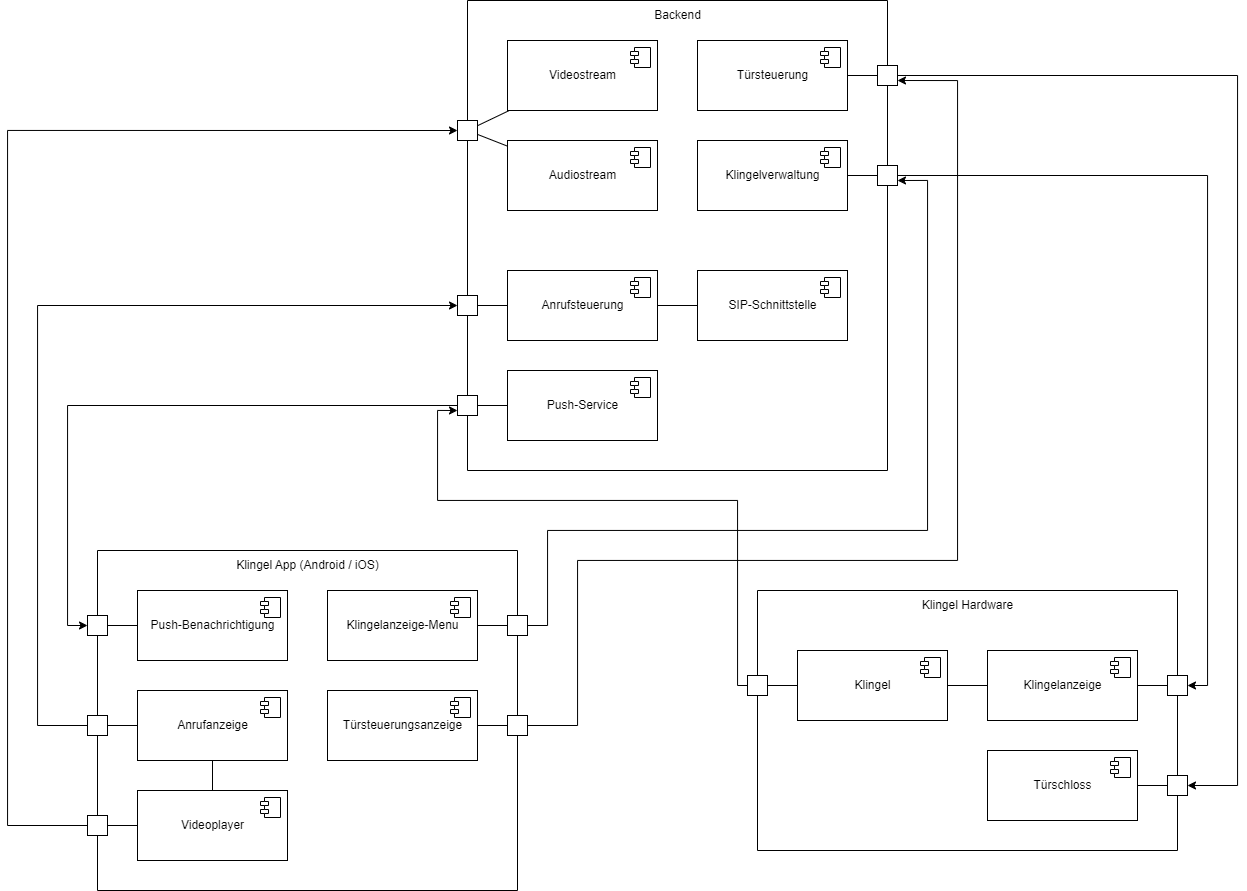
\includegraphics[width=\paperwidth-2in]{../assets/img/Komponentendiagramm}

    \caption{Komponenten von App, Hardware und Backend}
    \label{fig:komponentendiagramm}
\end{figure}
In Abbildung~\ref{fig:komponentendiagramm} ist das Komponentendiagramm dargestellt.
Dabei besteht die Klingel Hardware aus der Klingel selbst, die den Push-Service im Backend aktivieren muss 
und aus der Klingelanzeige, auf der nach Wunsch ein Name oder nur die Wohnungsnummer angezeit werden kann.
Außerdem ist die Türschloss-Komponente dafür da, die Tür auf- und zuzuschließen.

Das Backend wird um den Push-Service erweitert, der eine Push-Benachrichtigung senden kann.
Außerdem die Anrufsteuerung zum Steuern der Anrufe nach dem SIP-Standard.
Desweiteren gibt es im Backend die Audio- und Videostream Komponenten, die für die Anrufe selbst wichtig sind.
Diese können Audio und Video an die Klingel-App übertragen.
Die Türsteuerung ist dafür da das Türschloss zu kontrollieren und die Klingelverwaltung kann die Klingelanzeige in der Klingel-Hardware steuern.

Im dritten Subsystem, die Klingel-App, gibt es zum einen die Komponente der Push-Benachrichtigung.
Außerdem das Klingelanzeige-Menu, welche von der Klingelverwaltung eine Übersicht aller Klingeln anzeigen kann.
Die Türsteuerungsanzeige ist wesentlich die Visualisierung der Türsteuerung.
Zuletzt gibt es noch die Anrufanzeige in Verbindung mit dem Videoplayer, die jeweils mit Video- und Audiostream und der Anrufsteuerung im Backend komunizieren.
So kann der Benutzer den Anruf über die Visualisierung steuern und gegebenfalls das übertragene Video sehen.


\subsubsection{Requires / Provides}\label{subsubsec:requires-/-provides}
    \begin{figure}[ht!]
        \centering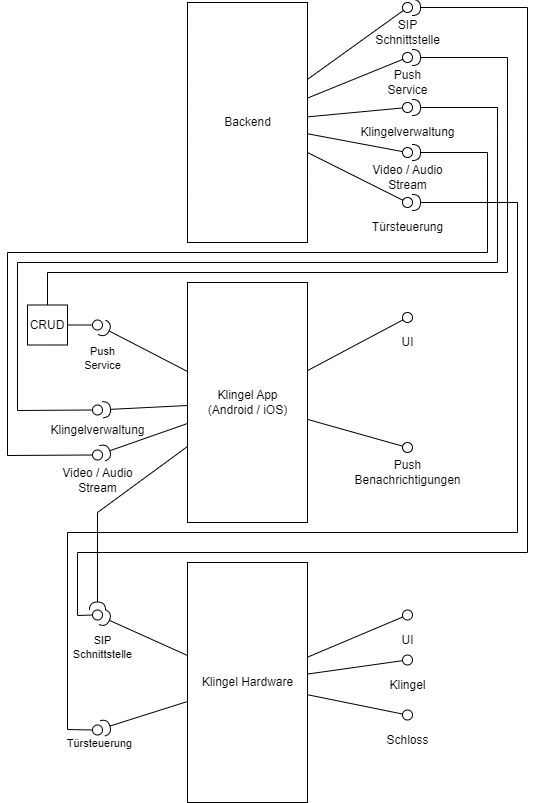
\includegraphics[width=\paperwidth/2]{../assets/img/requires_provides}

        \caption{Abhängigkeiten von App, Hardware und Backend}
        \label{fig:requires-provides}
    \end{figure}
    Das Backend, wie in Abbildung~\ref{fig:requires-provides} zu erkennen ist, hat, da es lediglich erweitert wird, keinen neuen Abhängigkeiten.
    Es werden nur ein paar neue Endpunkte bereitgestellt.
    Unter anderem ein paar CRUD Schnittstellen für die App, um die Klingeln zu verwalten, aber auch die Streams und SIP--Schnittstellen für die Telefonie werden bereitgestellt.
    App und Hardware konsumieren diese Schnittstellen und stellen im gegenzug das UI bereit.
    Eine direkte Verbindung gibt es dabei nicht.
    Das Backend dient als vermittler.


    Auch gibt es nur einen Adapter, von dem vom Backend bereitgestellten Push Service zu einer Push--CRUD--API\@.
    Der benötigte Adapter wird allerdings voraussichtlich in der Praxis teil des Backends, weshalb seine Existenz bestreitbar ist.
